\documentclass[11pt, oneside]{article} 
\usepackage{geometry}
\geometry{letterpaper} 
\usepackage{graphicx}
	
\usepackage{amssymb}
\usepackage{amsmath}
\usepackage{parskip}
\usepackage{color}
\usepackage{hyperref}

\graphicspath{{/Users/telliott_admin/Tex/png/}}
% \begin{center} 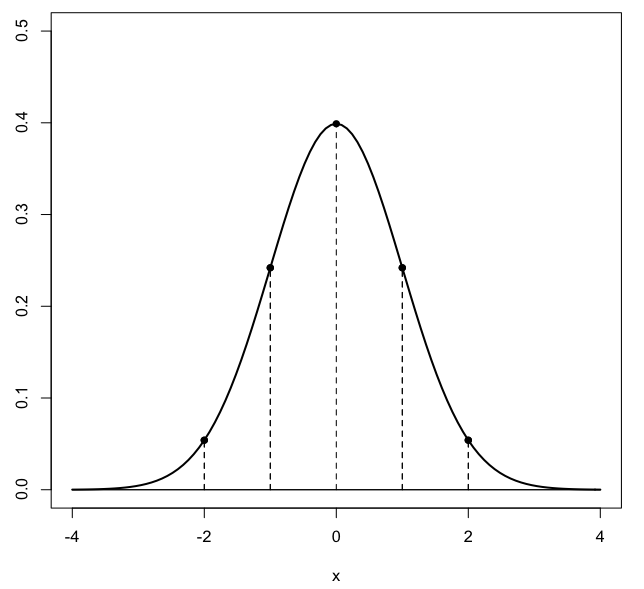
\includegraphics [scale=0.4] {gauss3.png} \end{center}

\title{Circular segment}
\date{}

\begin{document}
\maketitle
\Large

I found a hard geometry problem on the web:
\begin{center} 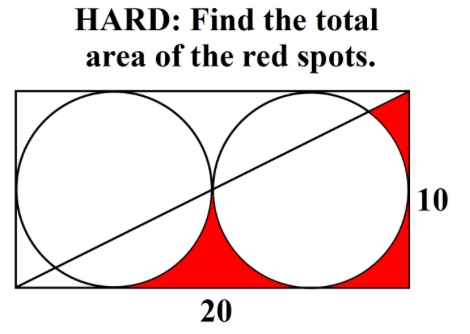
\includegraphics [scale=0.4] {circ_seg_prob.png} \end{center}
We know it's hard because it says so!

I liked it particularly because I found several different ways to calculate the answer, using basic geometry and trigonometry, and regular integration as well as polar integration.

As a first step, scale the problem down by a factor of $5$.  The two circles become unit circles, and then we'll re-scale the answer at the end, multiplying areas by $25$.

The area of an arched red segment in a corner is pretty easy, $4$ of them together are equal to the difference between the area of a square with side length $2$ and a unit circle:  $4 - \pi$, so each one is $1 - \pi/4$.

The real difficulty is the upper right-hand corner.
\begin{center} 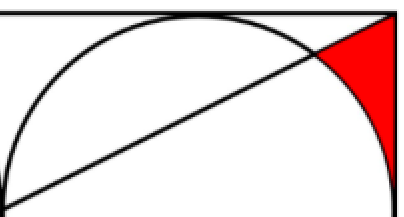
\includegraphics [scale=0.25] {circ_seg_prob2.png} \end{center}
One of the arches is divided into two pieces, and we are supposed to only count part of it.

The basic right triangle that we see repeated in these images has side lengths in the ratio $1:2$.  It's area is just $1$, and the smaller angle is 
\[ \phi = \tan^{-1} 0.5 \approx 0.4636 \text{ rad } \approx  26.565 \text{ deg } \]

\begin{center} 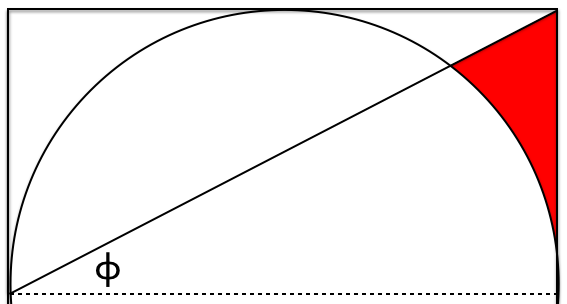
\includegraphics [scale=0.4] {circ_seg3.png} \end{center}
That's not a nice round number, but OK.
 
At first, it looked to me as if we need to calculate the area cut off by a chord of a circle, called a "circular segment".  

Then we could calculate the white part of the divided arch:
\[ \text{ triangle } - \text{ segment }  - \text{ arch } \]
\[ 1 - \text{ segment }  - (1 - \pi/4) \]

and subtract that from one whole arch to get the red part.
\[ (1 - \pi/4) - \ [ \ 1 - \text{ segment }  - (1 - \pi/4) \ ] \]
\[ 1 -  \frac{\pi}{2}  + \text{ segment } \]
We will use this result at the end for our final answer.

A circular segment is like a polar cap, but in two dimensions.
\begin{center} 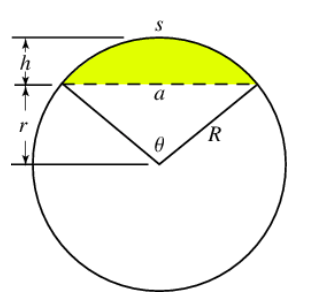
\includegraphics [scale=0.6] {circ_seg.png} \end{center}

\url{http://mathworld.wolfram.com/CircularSegment.html}

We carefully distinguish between the circular segment, in yellow, and the circular sector, which is the area of that slice of the circular pie swept out by the angle $\theta$.  That area is the fraction of the total circular angle, times the area of a unit circle, which is just half the angle.
\[ \frac{\theta}{2 \pi} \ \pi = \frac{\theta}{2} \]

For the actual calculation of a circular segment, we would need not only the angle $\theta$, but also $r$ and $a$, which we derive from $\theta$ by applying the Pythagorean theorem and/or trigonometry.  It can be done!  However, there is a simpler way.  

The first key idea to draw $\theta$ on our diagram, and realize that $\theta$ is the apex angle of an isosceles triangle because the two sides are radii of our circle and are equal to each other!  So $\theta = \pi - 2 \phi$.
\begin{center} 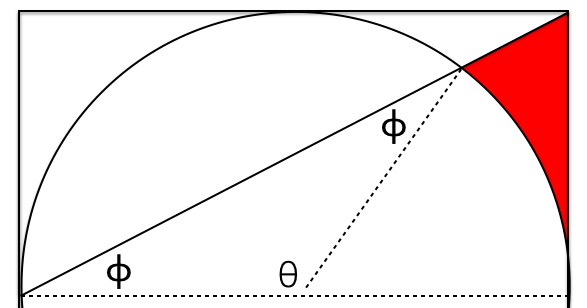
\includegraphics [scale=0.4] {circ_seg2.png} \end{center}

So now we calculate the circular sector swept out by $\theta$ and figure out the area of the isosceles triangle, subtract to find the spherical segment and be on our way.

\begin{center} 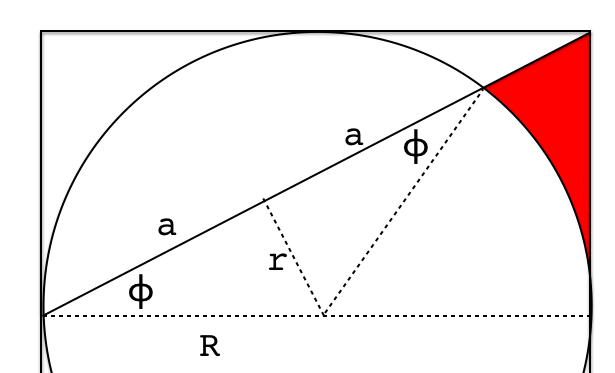
\includegraphics [scale=0.4] {circ_seg4.png} \end{center}
The triangle area is easy because one-half of it is a triangle similar to the original.  This means that $r/a = \tan \phi = 0.5$ so
\[ a = 2r \]
Furthermore
\[ r = R \sin \phi \]
\[ a = R \cos \phi \]

The area of the isosceles triangle is
\[ A = ar = R^2 \sin \phi \cos \phi \]
We can also do it solely in terms of $r$
\[ A = 2r^2 \]
\[ = 2 R^2 \sin^2 \phi \]
Recall that this is a unit circle so
\[ A = 2 \sin^2 \phi \]

This works because 
\[ \cos \phi = 2 \sin \phi \] 
so
\[  \sin \phi \cos \phi = 2 \sin^2 \phi \]

Because of the square we get an exact answer:
\[ \sin \phi = \frac{1}{\sqrt{5}} \]
\[ \sin^2 \phi = \frac{1}{5} \]
\[ A = 0.4 \]

Later, we will have a use for $h$:
\[ h = R - r = R(1 - \sin \phi) \]
\[ = 1 - \sin \phi \]

We could move on to consideration of the circular sector with angle $\theta$.  But wait!

Notice at this point a different circular sector, just to the right of the isosceles triangle.  Two different familiar theorems gives the angle as $2\phi$.
\begin{center} 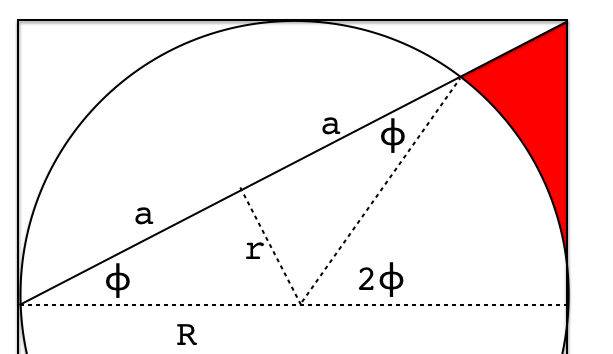
\includegraphics [scale=0.4] {circ_seg5.png} \end{center}
The area of that sector is, by the same calculation we did before, the ratio of the angle to $2 \pi$ times the area of the unit circle.
\[ \frac{2 \phi}{2 \pi} \ \pi = \phi \]

\subsection*{calculation 1:  ignore the circular segment}
So far we have that the area of the isosceles triangle is $2 \sin^2 \phi = \sin \phi \cos \phi$

The circular sector with angle $2 \phi$ has area $\phi$.

The part of the large lower triangle that is not in red is
\[ \text{ circular sector } + \text{ isosceles triangle } \]
\[ \phi + 2 \sin^2 \phi \]

Then what we want is to subtract that from the large triangle:
\[ A = 1 - \phi - 2 \sin^2 \phi \]
\[ = 1 - \approx 0.46 - 0.4 \]
I get $\approx 0.14$, which seems reasonable.  Remember that:  the red part of the arch is $1 - \phi - 2 \sin^2 \phi$.

\subsection*{calculation two:  polar area}
We can also use calculus, namely to compute a polar area.  Look again at
\begin{center} 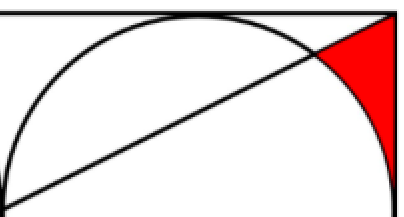
\includegraphics [scale=0.25] {circ_seg_prob2.png} \end{center}

What if we could get the area of the lower triangle minus the red part?

This is a pretty easy integral in polar coordinates.  Since the angle is usually given as $\theta$, for the moment we relabel $\phi$ as $\theta$.

Set up a circle of radius $a$ with its left edge at the origin, the equation of that circle in polar coordinates is
\[ r = 2 a \cos \theta \]

For example, radius $a = 1$ gives
\[ \text{at } \theta = 0, \ \ \ \ r = 2 \]
\[ \text{at } \theta = \frac{\pi}{4}, \ \ \ \ r = \sqrt{2} \]
\[ \text{at } \theta = \frac{\pi}{2}, \ \ \ \ r = 0 \]
The arc of the upper semi-circle that we're seeing is $\theta = 0 \rightarrow \frac{\pi}{2}$

You don't believe me that this is correct?  We have four equations.  Always:
\[ r^2 = x^2 + y^2 \]
\[ x = r \cos \theta  \]
\[ y = r \sin \theta  \]
\emph{Do not cancel} the $r = 1$ yet.

We also have the equation of this circle.  The general equation is
\[ r = 2h \cos \theta + 2k \sin \theta \]
where $(h,k)$ is the origin of the circle.  Here, the origin is at $h = 1$ so
\[ r = 2 \cos \theta \]

Now comes the magic.  Substitute for $\cos \theta $:
\[ r = 2 \frac{x}{r} \]
\[ r^2 = 2 x \]
but
\[ r^2 = x^2 + y^2  \]
We obtain
\[ x^2 + y^2 = 2x \]
\[ x^2 - 2x + y^2 = 0 \]
Complete the square and add the same term on the right
\[ (x - 1)^2 + y^2 = 1 \]
This is indeed a unit circle with origin at $(1,0)$.

\subsection*{polar area}

The area is made up of many small wedges with angle $\theta$, and $r = f(\theta) = 2 \cos \theta $.  The wedges are approximately triangles with area $1/2 \cdot r \cdot r \ d \theta$.  So the total area is

\[ A = \int \frac{1}{2} \ [ \ f(\theta) \ ]^2 \ d \theta \]

\[ = \frac{1}{2} \ 4 \int \cos^2 \theta \ d \theta\]
\[ = 2 \ [ \ \frac{1}{2} (\theta + \sin \theta \cos \theta) \ ] \ \bigg |_0^{\phi} \]
At the lower bound, this is zero so
\[ = \phi + \sin \phi \cos \phi \]
\[ = \phi + 2 \sin^2 \phi \]

This should be equal to the area of the circular sector of angle $2 \phi$ plus the area of the isosceles triangle, and if you look back, you'll see that we have a match.

To get the red arch, we must subtract this from the triangle, which has unit area.
\[ A = 1 - \phi - 2 \sin^2 \phi \]

That matches what we had before.  To finish up, we do this two more ways, both requiring the area of the circular segment.

\subsection*{calculation 3:  standard calculus}
We find the circular segment by standard integral calculus:

\begin{center} 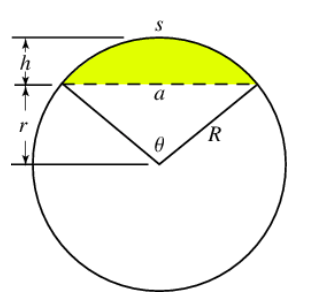
\includegraphics [scale=0.6] {circ_seg.png} \end{center}
Recall that the area of (the upper half of) a circle is
\[ \int \sqrt{R^2 - x^2} \ dx \]
The bounds we need are $R-h$ to $R$.

This is a unit circle so
\[ A = \int_{1-h}^1 \sqrt{1 - x^2} \ dx \]
The answer (done many times by now)
\[ \frac{1}{2} \ [ \ \sin^{-1} x + x \sqrt{1 - x^2} \ ]  \ \bigg |_{1-h}^1 \]

At the upper bound we get $\pi/4$.  For the lower bound we need $h$
\[ h = 1 - \sin \phi \]
so that bound is just $\sin \phi$.
The first term in parentheses is
\[ \sin^{-1} (\sin \phi) \]
The angle whose sine is $\sin \phi$ is just $\phi$!

The second term is
\[ (\sin \phi) \sqrt{1 - (\sin \phi)^2} \]
\[ = \sin \phi \cos \phi \]
Altogether, we have 
\[ \frac{\pi}{4} - \frac{1}{2} (\phi + \sin \phi \cos \phi) \]
\[ = \frac{\pi}{4} - \frac{\phi}{2} - \sin^2 \phi  \]
This is (almost) the circular segment.

It is off by a factor of 2.  The reason is that the integral only gives the area of that part of the circle that is above the $x$-axis.  We must multiply the provisional answer by $2$.
\[ = \frac{\pi}{2} - \phi - 2 \sin^2 \phi  \]

Wait for the calculation of the red part of the arch, starting from the circular segment.

\subsection*{calculation four:  geometry}

\begin{center} 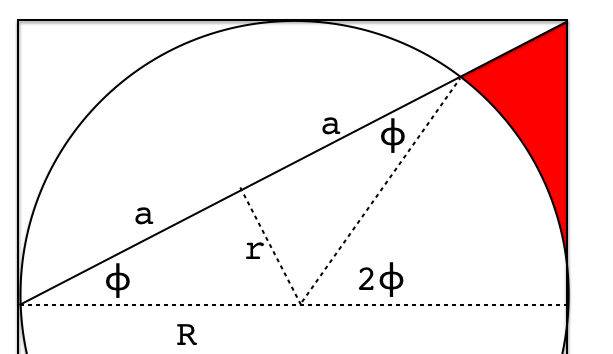
\includegraphics [scale=0.4] {circ_seg5.png} \end{center}
We have that the area of the isosceles triangle is exactly 
\[ \sin \phi \cos \phi = 2 \sin^2 \phi = 0.4 \]

The area of the circular sector with angle $\theta$ is 
\[ \frac{\theta}{2 \pi} \ \pi =  \frac{\theta}{2} \]
in terms of angle $\phi$:
\[ = \frac{1}{2} (\pi - 2 \phi) \]
\[ = \frac{\pi}{2} - \phi \]

The area of the circular segment is the area of the circular sector minus that of the isosceles triangle:
\[ \frac{\pi}{2} - \phi - 2 \sin^2 \phi \]
This matches what we had for the third calculation, by integration of the equation of the circle.

\subsection*{the red part of the arch}
At the very beginning we calculated the red part of the arch as:
\[ 1 -  \frac{\pi}{2}  + \text{ segment } \]

Now we have the circular segment with angle $\theta$ (in terms of $\phi$) as 
\[ \frac{\pi}{2} - \phi - 2 \sin^2 \phi \]

So the answer for the red part of the arch is
\[ 1 -  \frac{\pi}{2}  + \frac{\pi}{2} - \phi - 2 \sin^2 \phi \]
\[ 1 - \phi - 2 \sin^2 \phi \]

This matches parts one and two.  All four methods give the same answer, which is quite a relief.

\subsection*{finishing up}
To meet the problem statement, we must add this fractional arch to $3$ complete copies, and then multiply the whole thing by the square of the scaling factor (because this is an area):

\[ 25 \ [ 1 - \phi - 2 \sin^2 \phi \ + 3(1 - \pi/4) \ ] \]
I'm too tired to calculate it.

\begin{center} 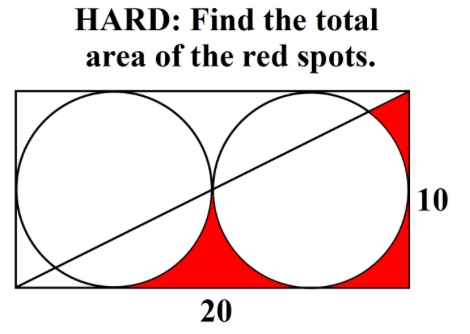
\includegraphics [scale=0.4] {circ_seg_prob.png} \end{center}

\end{document}